\section{Introduction}
\label{sec:introduction}

% challenge in multi-stage manipulation √
Sparse supervision is a key challenge in imitation learning, particularly for multi-stage robot manipulation tasks~\citep{Zare2024Survey,Mandlekar2020Learning,Chen2023Sequential,Jain2025LongerHorizon}. Completing such tasks requires a policy not only to understand the environment at the current time step, but also to retain knowledge of the past---for example, whether prior subtasks succeeded and how key objects changed (Figure~\ref{fig:teaser}, left)~\citep{Kang2025Incorporating,Mark2026BPP}. Because an environment consists of objects, the policy must understand how these objects have changed over time. Therefore, the currently observed environment alone is insufficient for the policy to predict the most appropriate action. The policy must also be aware of object changes within the environment. We refer to this challenge as the object-state transition supervision gap.
% Sparse supervision 在 imitation learning 中是一个 key challenge，特别是在 multi-stage robot manipulation 这一特定的 robot manipulation 任务类型中。
% multi-stage robot manipulation 在完成任务时，不仅仅需要 policy 理解当前时刻的 environment，还需要 policy 知晓过往的信息，比如上一个任务是否已经成功，之前执行任务时 environment 发生了哪些会影响当前任务执行的变化，而 environment 是由 object 组成的，也就是说 policy 需要知晓 object 在 environment 中一段时间下经历了哪些变化。
% 因此，仅仅只有当前观测到的 environment 不足以支撑 policy 预测最合理的动作，policy 还需要知晓 environment 中 object 的变化，我们称之为 object-state transition supervision gap

% how existing works solve this √
Early imitation learning methods improve short-term action prediction through action chunking or limited observation windows, but do not explicitly capture long-horizon task-relevant state transitions~\citep{Zhao2023Learning, chi2024diffusionpolicy}. Recent approaches incorporate past information through observation histories, latent memories, or task progress \citep{Liang2021Finite, shi2025memoryvla, Mark2026BPP}. Others use future observations, goal states, or latent plans as additional supervision \citep{lynch2020play, Mandlekar2020Learning, belkhale2023plato}. However, these methods represent temporal information at observation, latent, or task level, providing limited supervision on individual-object evolution during execution. Our method bridges this gap by unifying both temporal directions at the object level. Specifically, it represents past object-state transitions as structured historical context and predicts future object states as auxiliary supervision, enabling the policy to reason about how task-relevant objects have changed and how they should evolve next.

\begin{figure}[t]
    \centering
    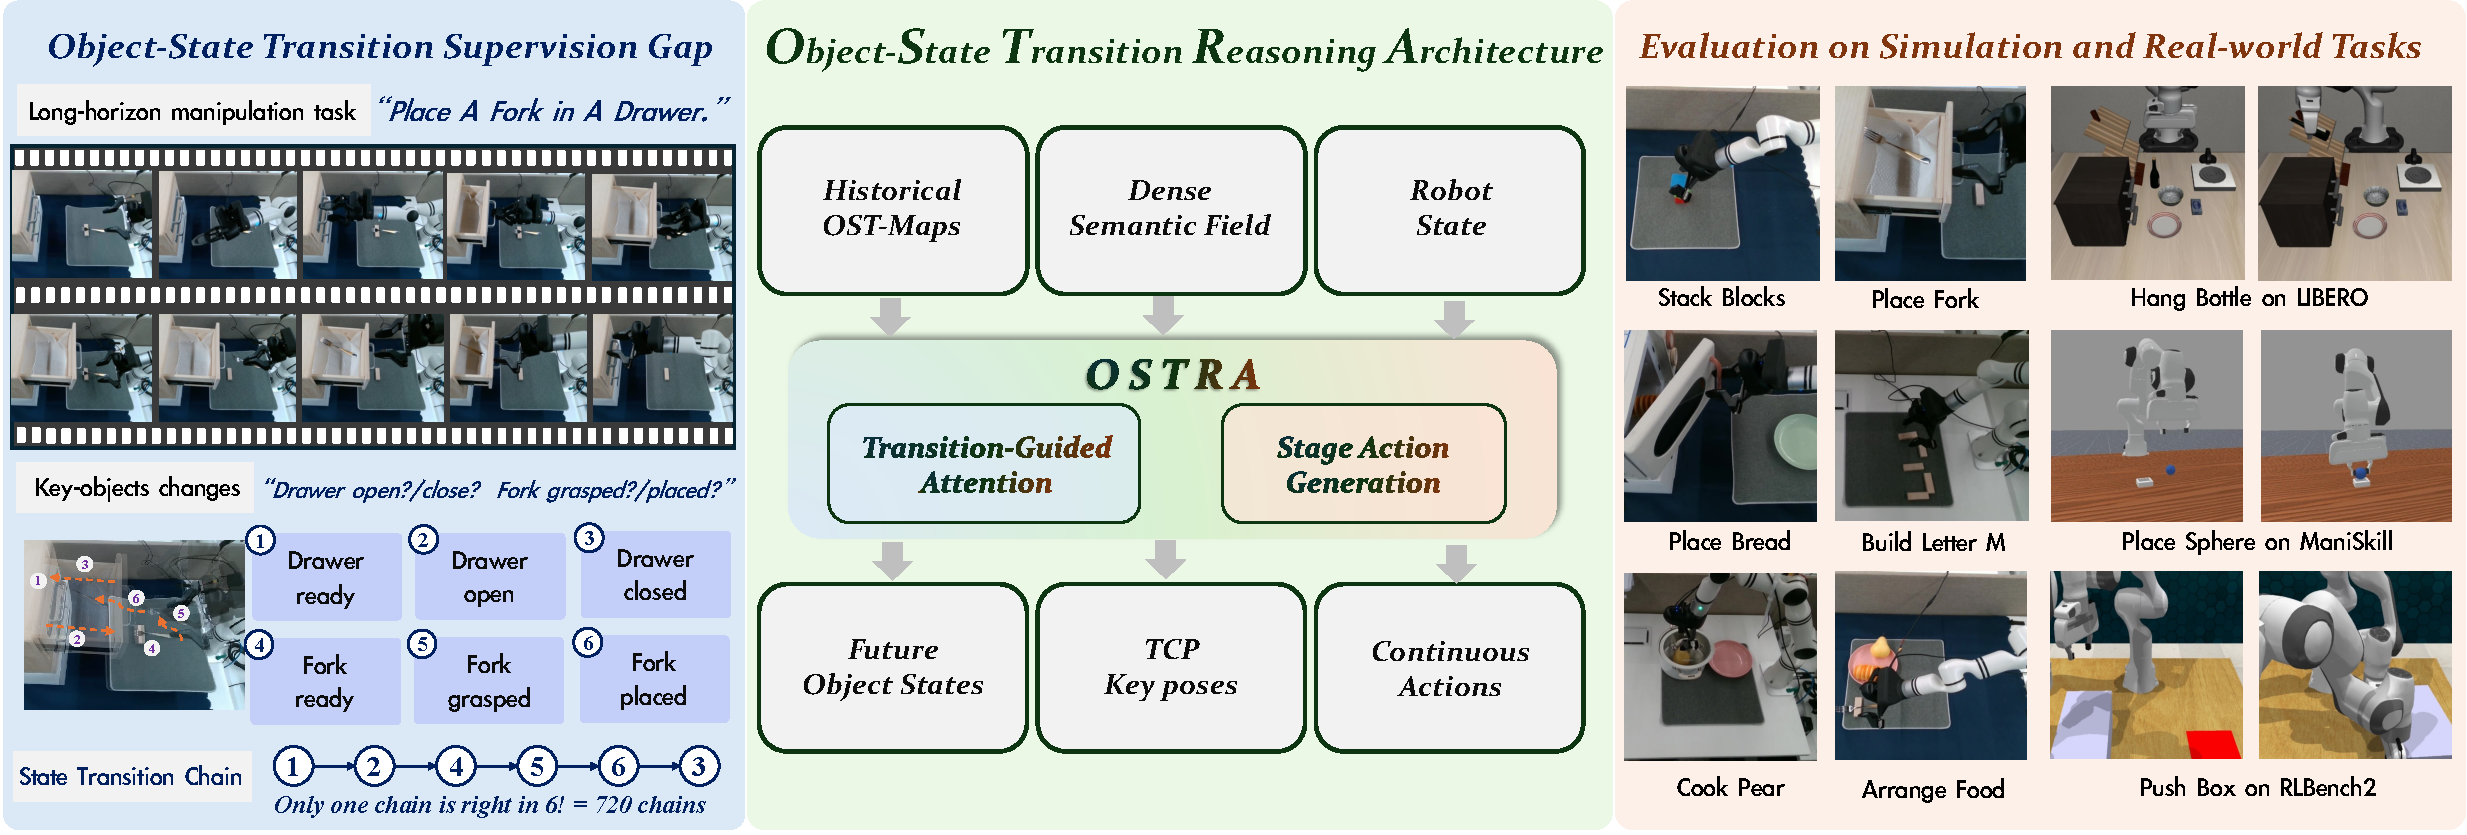
\includegraphics[width=\linewidth]{fig/1_teaser.pdf}
    \vspace{-20pt}
    \caption{\textbf{Overview of OSTRA.} Multi-stage manipulation requires
    resolving the object-state transition supervision gap: the policy must
    infer the correct transition chain from historical object changes. OSTRA
    combines historical OST-Maps, a dense Semantic Field, and the robot state
    to predict future object states, TCP keyposes, and continuous actions, and
    is evaluated across simulation and real-world tasks, where explicit
    transition supervision supports long-horizon control.}
    \vspace{-15pt}
    \label{fig:teaser}
\end{figure}



% OST-Map
To provide such supervision over past-to-future object evolution, we introduce the \textbf{O}bject-\textbf{S}tate \textbf{T}ransition Map (OST-Map), an object-centric representation of observed and future states in a shared structured space.
OST-Map avoids requiring policies to discover transition-relevant cues from visual histories using robot-centric action supervision alone.
Specifically, OST-Map represents each task-relevant object as an identity-consistent graph of structural nodes. Each node encodes its semantic identity, geometric parameters, and 6-DoF pose, while the graph edges capture structural and spatial relations among nodes and objects.
By preserving object and node identities across time, OST-Map organizes observations into temporally ordered object-centric tokens that explicitly characterize how task-relevant objects evolve. It further represents future object states in the same structured space, allowing the transition from historical to future object states to be directly supervised.
In this way, OST-Map turns otherwise implicit task progress and anticipated object changes into explicit intermediate targets between visual perception and robot action generation.

% OSTRA
Building on OST-Map, we introduce OSTRA, an \textbf{O}bject-\textbf{S}tate \textbf{T}ransition \textbf{R}easoning \textbf{A}rchitecture for multi-stage manipulation (Figure~\ref{fig:teaser}, middle).
OSTRA is a diffusion-based framework that hierarchically predicts future object states, target TCP poses, and continuous action trajectories.
It incorporates two key designs.
First, Transition-Guided Attention attends to historical OST-Map tokens before incorporating dense Semantic Field tokens, encouraging the model to prioritize task-relevant object-state transitions when predicting future states.
Second, Staged Denoising follows an object-to-TCP-to-action hierarchy that progressively translates predicted object-state changes into robot subgoals and executable actions.
Together, these designs connect object-level transition reasoning with robot-level planning and continuous control, enabling the policy to reason from how objects have changed to how they should evolve next and which actions should realize those changes.

We evaluate OSTRA on three simulation benchmarks and seven diverse real-world tasks.
Across these settings, OSTRA consistently improves over representative imitation learning baselines on multi-stage manipulation tasks.
Further ablation studies validate the contributions of OST-Map, Transition-Guided Attention, and Staged Denoising, demonstrating the effectiveness of structured object-state transition supervision for connecting scene evolution with robot action generation.

Our contributions are:
(1) To tackle the object-state transition supervision gap in multi-stage imitation learning, we introduce OST-Map, an object-centric representation that aligns historical object-state sequences with future object-state targets, enabling direct supervision of object-state transitions.
(2) Building on OST-Map, we introduce OSTRA, a diffusion-based architecture with two key designs.
    a) Transition-Guided Attention applies cross-attention to OST-Map tokens before Semantic Field tokens, encouraging the model to prioritize object-state transition information.
    b) Staged Denoising hierarchically predicts future object states, TCP poses, and action trajectories, progressively translating object-level state changes into robot subgoals and continuous control.
(3) We conduct evaluations across three simulation benchmarks and seven diverse real-world tasks, demonstrating consistent performance gains over representative imitation learning baselines.
% Further ablation studies validate the contributions of OST-Map, Transition-Guided Attention, and Staged Denoising, confirming the effectiveness of structured object-state transition supervision for multi-stage manipulation.
